

\chapter{Wstęp teoretyczny}
    \section{Klasyfikacje robotów}
    	\textbf{Robot mobilny} - robot, który potrafi zmieniać swoje położenie w przestrzeni. Może być robotem autonomicznym, czyli takim który realizując swoje zadanie porusza się bezkolizyjnie w wyznaczonym środowisku oraz robi to bez ingerencji operatora.
    	
    	Roboty mobilne można podzielić ze względu na ich mobliność:
    	\begin{itemize}
    		\item kołowe
    		\item kroczące
    		\item latające
    		\item pływające
    	\end{itemize}
    	Z kolei w robotach kołowych możemy rozróżnić następujące klasy:
    	\begin{itemize}
    		\item (3,0) - robot posiadający 3 koła szwedzkie. Najczęściej spotykany w formie trójkątnej platformy z przymocowanymi kołami do wierzchołków trójkąta. Jego zaletą jest możliwość poruszania się w dowolnym kierunku. Natomiast wadą trudne sterowanie.
    		\item (2,1) - robot posiada 2 koła kastora z tyłu oraz jedno obrotowe, napędowe z przodu. Zaletą jest prostota konstrukcji natomiast wadą trudne sterowanie oraz wrażliwość na nierówności terenu.
    		\item (2,0) - robot tzw. unicycle. Posiada 2 niezależnie napędzane koła, ustawione naprzeciwko siebie. Są one przymocowane na sztywno do ramy. Robot ten musi posiadać także punkt podparcia, którym najczęściej jest koło kastora. Plusami takiego rozwiązania jest prostota sterowania oraz konstrukcji. Dodatkowo robot posiada możliwość obrotu w miejscu. Minusem natomiast jest jego wrażliwość na nierówności.
    		\item (1,2) - robot posiada 2 koła napędowe, skrętne oraz jedno koło kastora służące za podporę. Konstrukcja wymaga zastosowania 3 silników, 2 do zmiany kąta każdego z kół oraz jeden napędowy. Tak więc minusem takiego rozwiązania jest jego skomplikowane sterowanie
    		\item (1,1) - robot nazywany także samochodem kinematycznym, ponieważ zachowuje się podczas sterowania jak zwykły samochód. Jego plusem jest niska wrażliwość na nierówności powierzchni, a jego minusem duży promień skrętu.
    	\end{itemize}
    	
    	Jedynym holonomicznym z wyżej wymienionych klas robotów mobilnych kołowym, jest klasa (3,0). Natomiast po uwzględnieniu wymagań stawianych robotowi zdecydowano się wybrać robota klasy (2,0). 
%	\textcolor{red}{Holonomiczność} - to w uproszczeniu brak ograniczeń na przeprowadzenie ruchu.

    \section{Kinematyka robota}
        Aby móc sterować robotem należy wyznaczyć kinematykę robota. Korzystając z wniosków zawartych w \cite{Mazur} można przyjąć, że klasa robotów (2,0) jest nieholonomiczna. To znaczy, że ruch takiego robota podlega pewnym ograniczeniom i nie wszystkie trajektorie mogą zostać zrealizowane. Autor wyjaśnia że, takie ograniczenia mogą wnikać z konstrukcji samego robota (wtedy są ograniczeniami wewnętrznymi). Przykładem może być ograniczenie skrętu układu kierowniczego. Ograniczenia mogą pochodzić również od otoczenia w którym robot się porusza. Takie ograniczenia noszą miano ograniczeń holonomicznych. Innym rodzajem ograniczeń są ograniczenia nieholonomiczne. Mamy do czynienia z nimi wtedy, gdy prędkości układu są ograniczone do liczby sterowań %\textcolor{red}{(w literaturze podawane jako (n - k) w macierzy Pfaffa ale to chyba to samo?)}
        przy braku ograniczeń konfiguracji układu. Przykładem może być parkowanie równoległe samochodu. Nie jesteśmy w stanie przesunąć auta prostopadle do drogi (ograniczenie) ale możemy odpowiednio nim sterując zaparkować (osiągnąć dostępną konfigurację).

        Zarówno ograniczenia holonomiczne jak i nieholonomiczne można przedstawić w postaci Pfaffa \ref{eq:ograniczeniaPfaffa}.
        
        \begin{equation}
            A(q)\dot{q}=0,
            \label{eq:ograniczeniaPfaffa}
        \end{equation}
        
        gdzie:
        
        \begin{itemize}
            \item[] $A(q)$ - macierz pełnego rzędu
            \item[] $q(t)$ - trajektoria układu
        \end{itemize}
        
        Dla robotów mobilnych kołowych ograniczenia nieholonomiczne w tej postaci wynikają z przyjętych założeń o braku poślizgu kół w miejscu ich styku z podłożem. Opierając obliczenia na \cite{Mazur} i \cite{Cholewinski} Dla monocykla można przyjąć:
        \begin{itemize}
            \item Ograniczenie ruchu poprzecznego (poślizg prostopadły do kierunku ruchu) \newline
                Wyrażone w postaci równania \ref{eq:ograniczeniePoprzeczne}
            \item Ograniczenie ruchu wzdłużnego (boksowanie kół) \newline
                Wyrażone osobno dla lewego i prawego koła przedstawiono w postaci równań \ref{eq:ograniczenieWzdloznePrawe} oraz \ref{eq:ograniczenieWzdlozneLewe}.
        \end{itemize}
        Schematy ideowe zostały pokazane na rysunku \ref{fig:monocykSchemat}.
    	\begin{figure}[ht]
			\centering
			\begin{tabular}{@{}ll@{}}
				a) & b) \\
				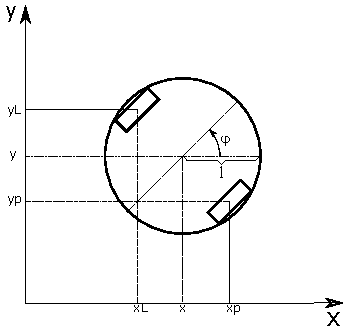
\includegraphics[width=0.5\textwidth]{rys01/rysunek.pdf} & 
				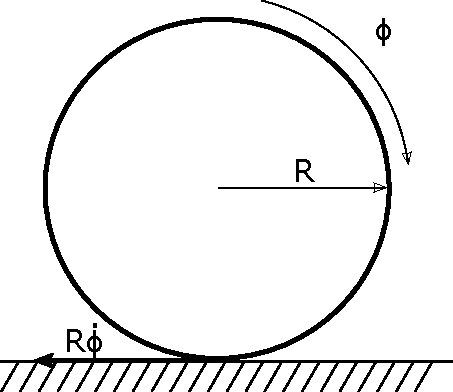
\includegraphics[width=0.4\textwidth]{rys02/kolo.pdf} \\
			\end{tabular}
			\caption{Schematy: a) monocykla i b) koła}
			\label{fig:monocykSchemat}
		\end{figure}
    	
        \begin{equation}
            \dot{x}\sin(\varphi) - \dot{y}\cos(\varphi) = 0
            \label{eq:ograniczeniePoprzeczne}
        \end{equation}
        \begin{equation}
            \dot{x}_L\cos(\varphi) + \dot{y}_L\sin(\varphi) - R\dot{\phi_1} = 0
            \label{eq:ograniczenieWzdlozneLewe}
        \end{equation}
        \begin{equation}
            \dot{x}_P\cos(\varphi) + \dot{y}_P\sin(\varphi) - R\dot{\phi_2} = 0
            \label{eq:ograniczenieWzdloznePrawe}
        \end{equation}
        Równania \ref{eq:ograniczenieWzdloznePrawe} i \ref{eq:ograniczenieWzdlozneLewe} można przedstawić we współrzędnych globalnych \ref{eq:ograniczenieWzdloznePraweGlobalne} i \ref{eq:ograniczenieWzdlozneLeweGlobalne}.
        \begin{equation}
            \dot{x}\cos(\varphi) + \dot{y}\sin(\varphi) -l\dot{\varphi} - R\dot{\phi_1} = 0
            \label{eq:ograniczenieWzdloznePraweGlobalne}
        \end{equation}
        \begin{equation}
            \dot{x}\cos(\varphi) + \dot{y}\sin(\varphi) +l\dot{\varphi} - R\dot{\phi_2} = 0
            \label{eq:ograniczenieWzdlozneLeweGlobalne}
        \end{equation}
        Robota przedstawionego w współrzędnych globalnych można przedstawić za pomocą wektora położeń %\ref{eq:wektorPolozen}.
        \begin{equation*}
            q =
            \begin{matrix}
                 ( x & y & \varphi & \phi_1 & \phi_2)
            \end{matrix}
            ^T\in R^5
            %\label{eq:wektorPolozen}
        \end{equation*}
        Który po zróżniczkowaniu daje wektor prędkości \ref{eq:wektorPredkosci}.
        \begin{equation}
            \dot{q} = 
            \begin{matrix}
                (\dot{x} & \dot{y} & \dot{\varphi} & \dot{\phi}_1 & \dot{\phi}_2)
            \end{matrix}
            ^T \in R^5
            \label{eq:wektorPredkosci}
        \end{equation}
        Z kolei ograniczenia \ref{eq:ograniczeniePoprzeczne}, \ref{eq:ograniczenieWzdloznePraweGlobalne} i \ref{eq:ograniczenieWzdlozneLeweGlobalne} można wyrazić w postaci macierzy ograniczeń Pfaffa \ref{eq:macierzPfaffa}.
        %\textcolor{red}{Błąd w ograniczeniach poprawić obliczenia}
        \begin{equation}
            A(q) =
            \begin{bmatrix*}[r]
            sin(\varphi) & -cos(\varphi) & 0  &  0 & 0 \\
            cos(\varphi) & sin(\varphi)  & -l & -R & 0 \\
            cos(\varphi) & sin(\varphi)  & l  &  0 & -R 
            \end{bmatrix*}
            \label{eq:macierzPfaffa}
        \end{equation}
        \textcolor{red}{Szerzej Wyjaśnić pominięcie ograniczenia poprzecznego}
        Dla robota mobilnego klasy (2,0) można pominąć ograniczenie ruchu poprzecznego \ref{eq:ograniczeniePoprzeczne}. Wynika to z m.in z faktu, że robot jest w stanie wykonać obrót w miejscu i osiągnąć zadaną pozycję. Wtedy możemy pominąć pierwszy wiersz macierzy \ref{eq:macierzPfaffa}. Przyjmuje ona wtedy postać \ref{eq:macierzPfaffaBezPoprzecznego}.
        \begin{equation}
            A(q) =
            \begin{bmatrix*}[r]
            cos(\varphi) & sin(\varphi)  & -l & -R & 0 \\
            cos(\varphi) & sin(\varphi)  & l  &  0 & -R 
            \end{bmatrix*}
            \label{eq:macierzPfaffaBezPoprzecznego}
        \end{equation}
        Dopuszczalne prędkości można wyrazić jako kombinację wektorów rozpinających jądro macierzy $A(q)$. Wektory te dają macierz $G(q)$, którą oblicza się z równania \ref{eq:obliczanieG}.
        \begin{equation}
            A(q)G(q)=0,
            \label{eq:obliczanieG}
        \end{equation}
        Następnie można zdefinować bezdryfowy układ sterowania w postaci \ref{eq:bezdryfowyUkladSterowania}.
        \begin{equation}
            \dot{q} = G(q)\eta
            \label{eq:bezdryfowyUkladSterowania}
        \end{equation}
        Który po uwzględnieniu ograniczeń \ref{eq:macierzPfaffa} przyjmuje postać \ref{eq:bezdryfowyUkladSterowaniaMonocykla}. \textcolor{red}{Sprawdzić poprawność macierzy G}
        \begin{equation}
            \dot{q} = G(q)\eta =
            \begin{bmatrix*}
                cos(\varphi) & cos(\varphi) \\
                sin(\varphi) & sin(\varphi) \\
                \frac{1}{l} & -\frac{1}{l} \\
                \frac{2}{R} & 0 \\
                0 & \frac{2}{R} 
            \end{bmatrix*}
            \left(\begin{array}{c}
                \eta_1 \\
                \eta_2
            \end{array}\right)
            \label{eq:bezdryfowyUkladSterowaniaMonocykla}
        \end{equation}
        Z dwóch ostatnich równań wynika, że prędkości $\eta$ są jedynie przeskalowanymi prędkościami kół
        \begin{equation*}
            \dot{\phi}_1 = \frac{2}{R}\eta_1, \quad \dot{\phi}_2 = \frac{2}{R}\eta_2
        \end{equation*}
        Dzięki temu kinematykę da się przedstawić w analogicznej formie \ref{eq:kinematykaDrugaForma}.
        \begin{equation}
            \left(\begin{array}{c}
                \dot{x} \\
                \dot{y} \\
                \dot{\varphi}
            \end{array}\right)
            =
             \begin{bmatrix}
                cos(\varphi) & 0 \\
                sin(\varphi) & 0 \\
                0 & 1
            \end{bmatrix}
            \left(\begin{array}{c}
                v \\
                \omega
            \end{array}\right)
            \label{eq:kinematykaDrugaForma}
        \end{equation}
        gdzie: \newline
        $v = \frac{R}{2}(\dot{\phi}_1+\dot{\phi}_2)$ -- prędkość postępowa robota \newline
        $\omega = \frac{R}{2l}(\dot{\phi}_1-\dot{\phi}_2)$ -- prędkość kątowa robota \newline
        Celem robota będzie śledzenie zadanej trajektorii dopuszczalnej, którą dla kinematyki w postaci \ref{eq:kinematykaDrugaForma} można przedstawić jako \ref{eq:generatorTrajektorii}.
        \begin{equation}
            \left(\begin{array}{c}
                \dot{x_d} \\
                \dot{y_d} \\
                \dot{\varphi_d}
            \end{array}\right)
            =
            \left(\begin{array}{c}
                v_{d}cos(\varphi_{d}) \\
                v_{d}sin(\varphi_{d}) \\
                \omega_{d}
            \end{array}\right)
            \label{eq:generatorTrajektorii}
        \end{equation}
        Prędkości liniowa $v_{d}$ oraz kątowa $\omega_{d}$ zawierają prędkości które powinien mieć układ aby podążał po zadanej trajektorii $(x_{d}, y_{d}, \varphi_{d})$. Następnie, aby móc realizować algorytm sterowania należy zdefiniować referencyjne błędy sterowania \ref{eq:referencyjneBledySterowania}.
        \begin{equation}
            \left(\begin{array}{c}
                x_{e} \\
                y_{e} \\
                \varphi_{e}
            \end{array}\right)
            = Rot(Z, -\varphi) 
            \left(\begin{array}{c}
                e_{x} \\
                e_{y} \\
                e_{\varphi}
            \end{array}\right)
            =
            \begin{bmatrix}
                cos(\varphi) & sin(\varphi) & 0 \\
                -sin(\varphi) & cos(\varphi) & 0 \\
                0 & 0 & 1
            \end{bmatrix}
             \left(\begin{array}{c}
                x_{d} - x \\
                y_{d} - y \\
                \varphi_{d} - \varphi
            \end{array}\right)
            \label{eq:referencyjneBledySterowania}
        \end{equation}
        Mając zdefiniowane referencyjne błędy sterowania można przedstawić algorytm sterowania w postaci algorytmu Samsona \ref{eq:algorytmSamsona}.
        \begin{equation}
            \left(\begin{array}{c}
                v_{r} \\
                \omega_{r} 
            \end{array}\right)
            =
            \left(\begin{array}{c}
                k_{1}x_{e} + v_{d}cos(\varphi_{e}) \\
                \omega_{d} + k_{2}\varphi_{e} + v_{d}y_{e}\frac{sin(\varphi_{e})}{\varphi_{e}}
            \end{array}\right)
            \label{eq:algorytmSamsona}
        \end{equation}
        Za $\frac{sin(\varphi_{e})}{\varphi_{e}}$ przyjęto wartość $1$.
    \section{Sterowanie silnikiem DC}
    	Do sterowania kierunkiem obrotów silnika szczotkowego DC wykorzystuje się układ zwany mostkiem H. Jest on przedstawiony schematycznie na rysunku \ref{fig:mostekHschemat}. 
    	
    	\begin{figure}[ht]
    		\centering
    		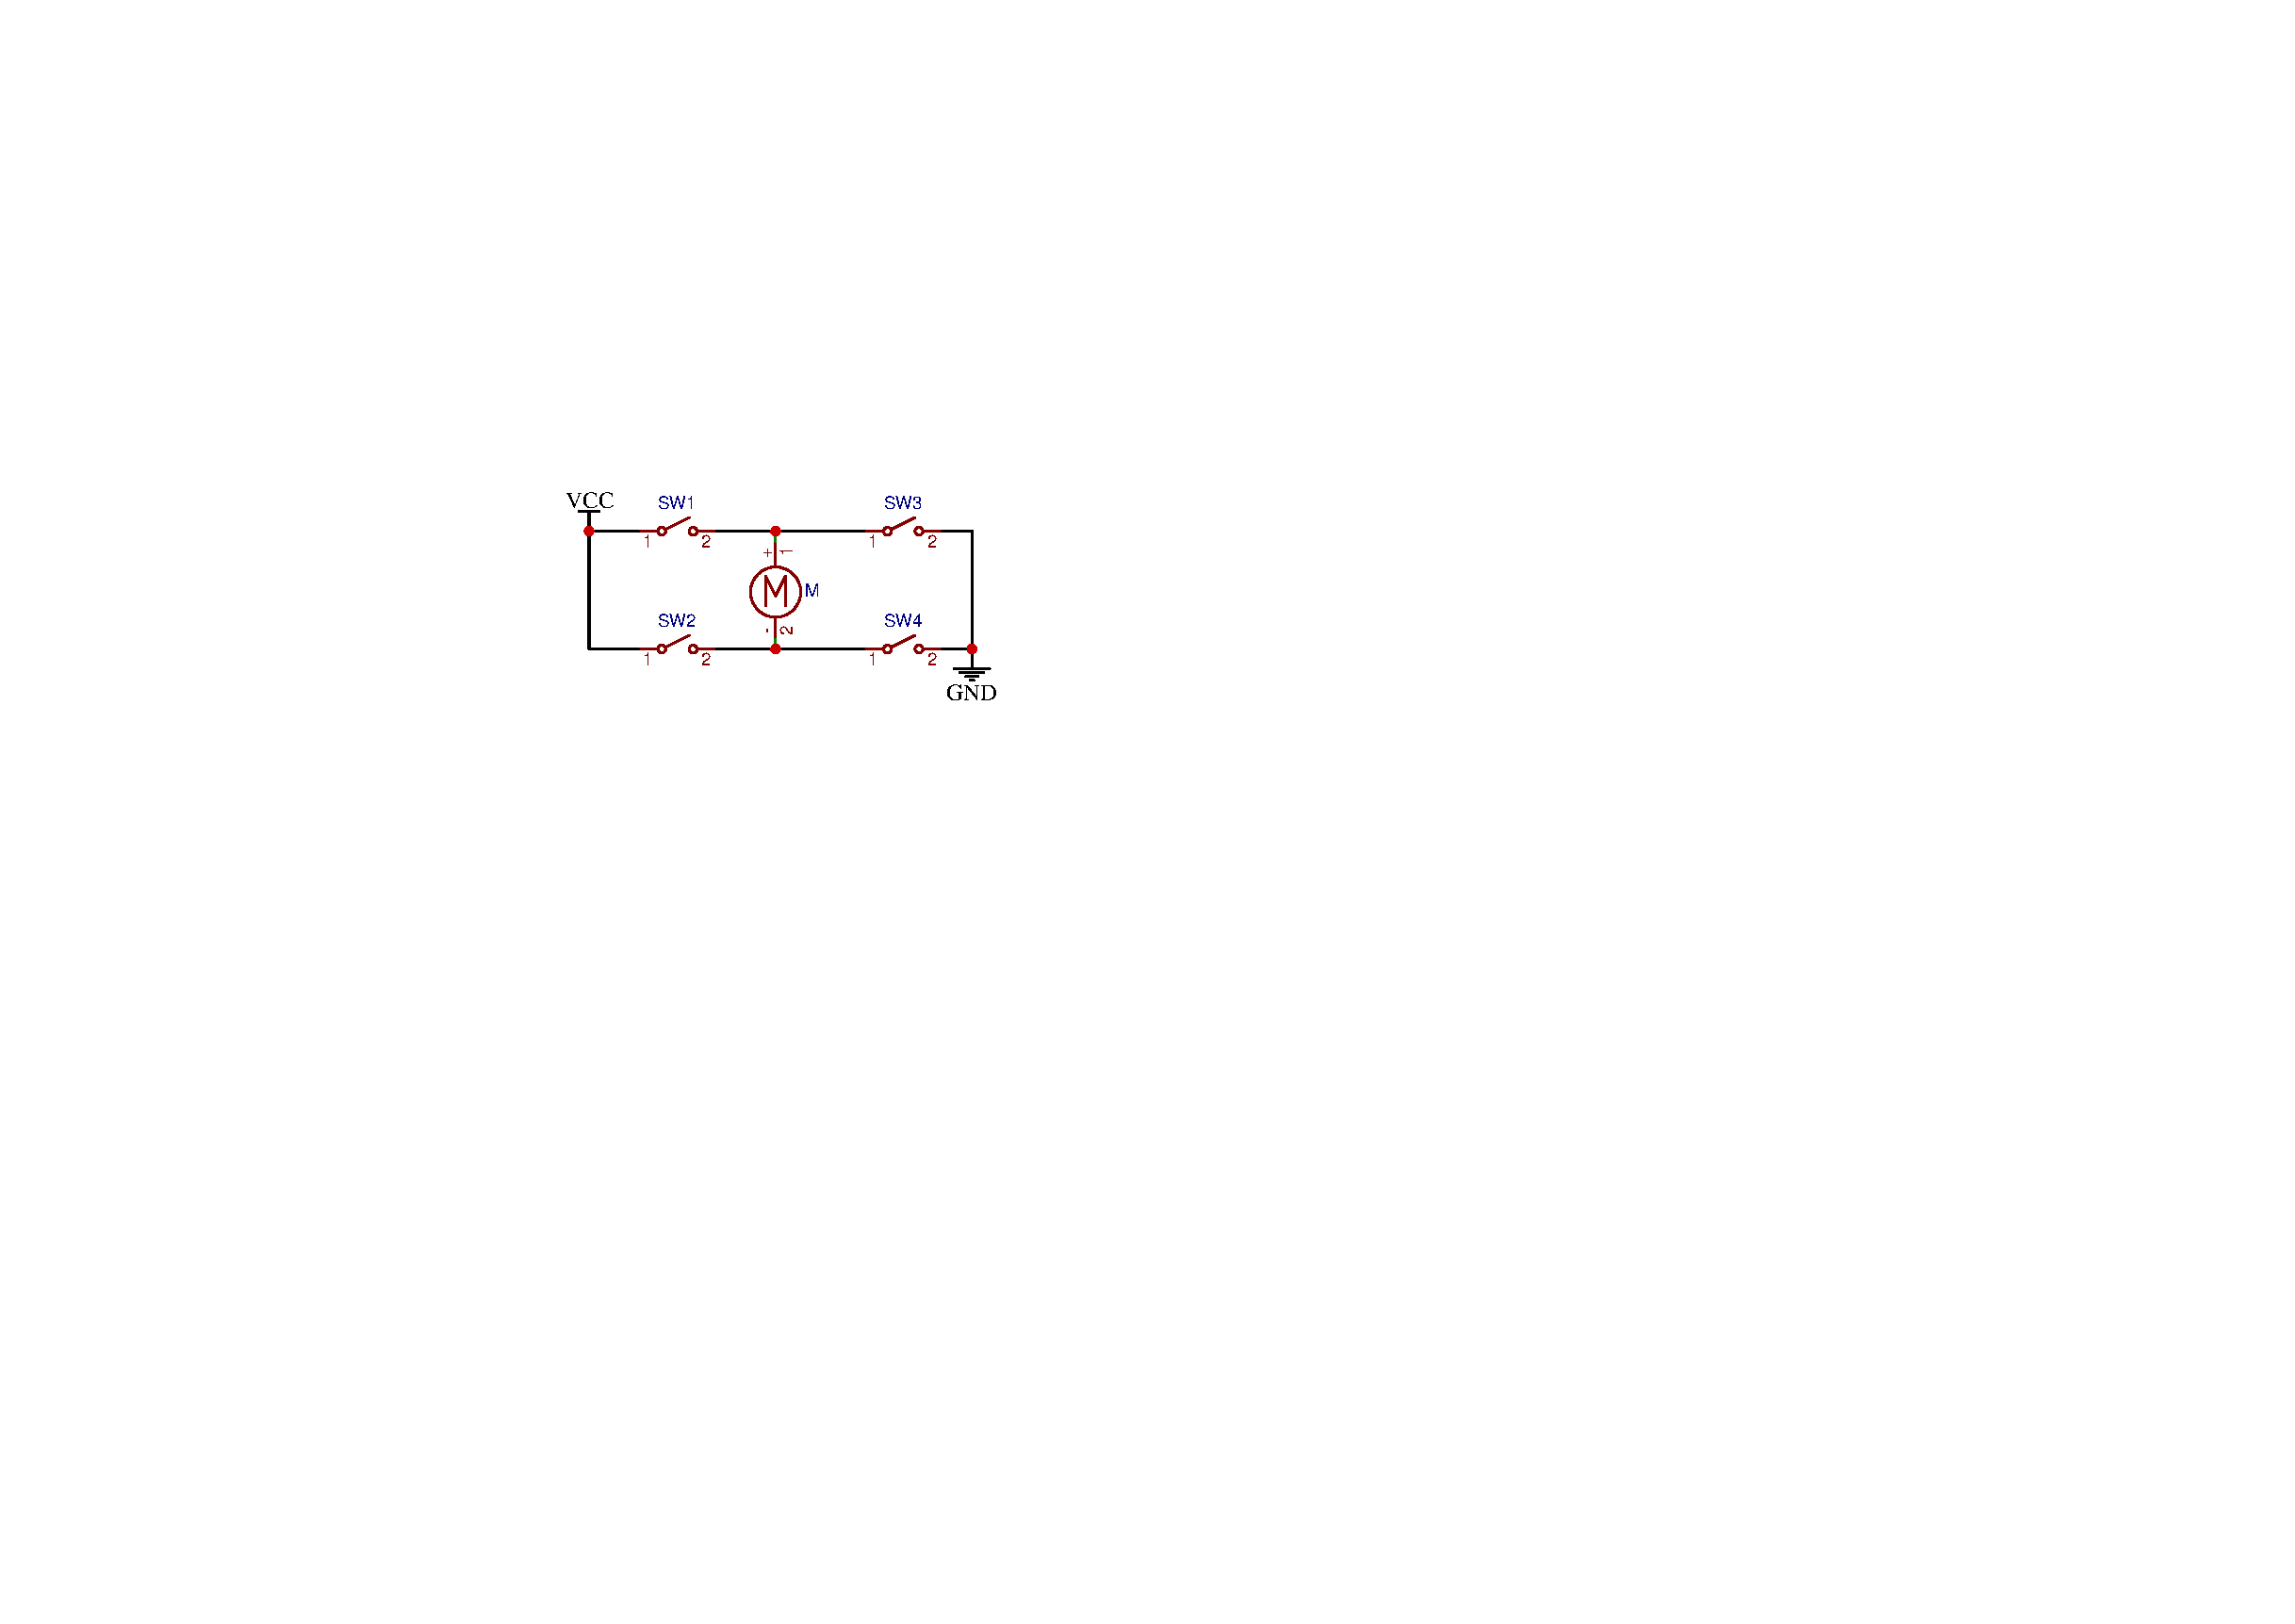
\includegraphics[width=0.6\textwidth]{rys02/mostekH.pdf} 
    		\caption{Schemat mostka H}
    		\label{fig:mostekHschemat}
    	\end{figure}
    
    	Styki oznaczone literą S i silnik oznaczony literą M przypominają kształt dużej litery H. Jego działanie polega na zwieraniu odpowiednio styków S1 oraz S4, aby uzyskać kierunek obrotów w jedną stronę. Chcąc uzyskać obroty w drugą stronę należy zewrzeć styki S2 i S3. Należy mieć na uwadze odpowiednie sterowanie, ponieważ załączenie w jednym czasie styków S1 i S3 lub S2 i S4 spowoduje zwarcie.
    	
    \section{Optymalizacja kodu}
    W projekcie wykorzystany został kompilator GNU. Posiada on możliwości optymalizacji kodu wynikowego. Przykładowe flagi optymalizacji przedstawione zostały w tabeli \ref{tab:optynalizacja}.
    \begin{table}[ht]
		\centering
		\begin{tabular}{|l|l|} \hline
			\textbf{Flaga} & \textbf{Działanie} \\
			\hline
			\hline  -O0 &  brak optymalizacji \\
			\hline  -Os &  optymalizacja rozmiaru kodu\\
			\hline 	-O1 &  optymalizacja czasu wykonywania\\
			\hline 	-O2 &  większa optymalizacja czasu wykonywania (zawiera -O1)\\
			\hline  -O3 &  jeszcze większa optymalizacja czasu wykonywania (zawiera -O2)\\
			\hline 	-Ofast & optymalizacja z pominięciem ścisłych standardów (zawiera -O3)  \\
			\hline
		\end{tabular}
		\caption{Flagi optymalizacji kodu kompilatora GNU}
		\label{tab:optynalizacja}
	\end{table}
	Często stosowaną flagą optymalizacji na mikrokontrolerów jest -Os. Jednak procesor użyty w tym projekcie posiada wystarczającą ilość pamięci, dlatego zdecydowano się użyć opcji -O3. Pozwoli to zoptymalizować czas obliczeń i skrócić czas wykonywania pętli programu. Szczegółowy opis wymienionych opcji znajduje się na stronie \cite{flagiGNUstrona}.
%%%
%%%Uwaga: tytuł powinien zmieścić się w okienku kolorowej okładki (którą
%%%powinna dostarczyć uczelniana administracja). Proszę posterować
%%%parametrami, aby "wpasować" w okienko własny tekst.
%%%
%%%Do ASAPa należy wprowadzić pracę dyplomową/projekt inżynierski w pliku o nazwie:
%%%
%%%W04_[nr albumu]_[rok kalendarzowy]_[rodzaj pracy] (szczegółowa instrukcja pod adresem asap.pwr.edu.pl)
%%%
           %%%Przykładowo:
        %%%­W04_123456_2015_praca inżynierska.pdf     - praca dyplomowa inżynierska
        %%%W04_123456_2015_projekt inżynierski.pdf   - projekt inżynierski
        %%%W04_123456_2015_praca magisterska.pdf  - praca dyplomowa magisterska
%%%
              %%%rok kalendarzowy ? rok realizacji kursu „Praca dyplomowa” (nie rok obrony) 